\chapter{Security and Performance Analyses}
\label{cha:5_analysis}
\parskip=0ex

In this chapter, security analysis of the proposed firmware update framework and protocol are provided and discussed. There is security analysis against attack within information exchange over insecure connection described in Section~\ref{sec:securityOverInsecure}. In the Section \ref{sec:protocolAnalysisTool} discussed how we use the analysis tools and the result. Performance analysis also conducted in Section~\ref{sec:performance} to compare the performance of the proposed protocol against existing firmware update protocol. In last section, Section~\ref{sec:discussion} summary the security analysis result from the previous sections.

% \begin{tabular}{@{}c@{}}\textbf{Peer-to-peer} \\ \textbf{firmware file sharing}\end{tabular}

\begin{table}[htb]
	\caption{Architecture design comparison of four blockchain-based firmware update framework}
	\label{tab:architectureComparison}
	\begin{adjustbox}{max width=1\textwidth,center}
		\begin{tabular}{|l|l|l|l|l|}
			\hline
			\textbf{Architecture design} & \textbf{Proposed framework} & \textbf{Yohan et al.~\cite{yohan}} & \textbf{Lee et al.~\cite{lee}} & \textbf{Boudguiga et al.~\cite{lee}}\\ \hline
			\textbf{Firmware update method} & Push-method & Push-method & Pull-method & Pull-method\\ \hline
			\textbf{Vendor platform} & Multiple vendors & Multiple vendors & Single vendor & Multiple vendors\\ \hline
			\textbf{IoT device platform} & Heterogeneous devices & Heterogeneous devices & Specific device & Heterogeneous devices\\ \hline
			\begin{tabular}{@{}l@{}}\textbf{Peer-to-peer firmware} \\ \textbf{ file sharing}\end{tabular} & Not allowed & Not allowed & Allowed & Allowed\\ \hline
			\textbf{Blockchain platform} & Skipchain & Ethereum & Bitcoin & Bitcoin\\ \hline
			\textbf{Smart Contract} & Available & Available & Not available & Not available\\ \hline
			\textbf{Trusted node} & Not-required & Not-required & Not-required & Required\\ \hline
			\textbf{Peer-to-peer verification} & Yes & No & No & No\\ \hline
		\end{tabular}
	\end{adjustbox}
\end{table}

Our proposed framework uses push-method to distribute the updated firmware, where a vendor can publish an update and notify the targetted device within the blockchain network without specific request from the device. The other two blockchain-based firmware achitectures~\cite{lee,boudguiga} applied pull-method, where an IoT device needs to send a firmware update request to check for the new available firmware version. Push-method can reduce attack-window time by updating the firmware immediately after the vendor publishes a new firmware update. Push-method is also more energy and network efficient than pull-method, because in pull-method, power-constrained and connection-limited IoT devices need to constantly request the availability of the new firmware version whether it is exist or not.

Our framework achitecture adopts skipchain technology, which enables smart contract creation. Skipchain as permissioned blockchain platform protocols adapts PBFT concept in the consensus mechanism. In our proposed framework, PBFT is a better choice because the framework does not allow anyone to join the blockchain network but only for registered vendor and gateway. PBFT tackle the energy required by proof-of-work consensus mechanism with drawback of no anonimity within the permissioned blockchain network.

Our proposed framework is able to provide peer-to-peer skipblock verification process by using the skipchain technology's forward link. It means that low-power with little or no Internet connectivity device does not need to maintain connections with many other network nodes. Low-power device can get the up-to-date block data from the stronger device (e.g gateway) via peer-to-peer connection, and securely verify if the new block data is exist in the valid skipchain network without storing the whole blockchain data.

\begin{table}[htb]
	\caption{The comparison of security mechanism against cyber attack of four blockchain-based firmware update framework}
	\label{tab:securityComparison}
	\begin{adjustbox}{max width=1\textwidth,center}
		\begin{tabular}{|l|l|l|l|l|}
			\hline
			\textbf{Provide protection against} & \textbf{Proposed framework} & \textbf{Yohan et al.~\cite{yohan}} & \textbf{Lee et al.~\cite{lee}} & \textbf{Boudguiga et al.~\cite{lee}}\\ \hline
			\textbf{Firmware modification attack} & Yes & Yes & No & Yes\\ \hline
			\textbf{Impersonation attack} & Yes & Yes & No & Yes\\ \hline
			\textbf{Man-in-the-middle attack} & Yes & Yes & Yes & Not specified\\ \hline
			\textbf{Replay attack} & Yes & Yes & Yes & Not specified\\ \hline
			\textbf{Isolation attack} & Yes & No & No & No\\ \hline
		\end{tabular}
	\end{adjustbox}
\end{table}

The comparison of the security mechanism between proposed framework and the other related works is shown in Table~\ref{tab:securityComparison}. Our proposed framework is designed to protect the firmware update process from major cyber-attack, respectively: firmware modification attack, impersonation attack, man-in-the-middle attack, replay attack and isolation attack. On the other hand, the firmware update mechanism proposed by Lee et al.~\cite{lee} could not prevent firmware modification and impersonation attack. Furthermore, our proposed framework provides additional security measure against isolation attack.

By nature, an offline blockchain node can not resist isolation attack, because there is no cryptographic means for any node to distinguish the real blockchain from a fake one. If an attacker can isolate (even temporarily) a node from the network, attacker can tricks the isolated node to accept the fake firmware update from newer block that never exist.

\section{Informal Security Analysis} 
\label{sec:securityOverInsecure}

The following theorems are applied on both firmware verification protocol and peer-to-peer verification protocol. \textbf{Vendor repository} roles in firmware verification protocol and \textbf{IoT devices} roles in peer-to-peer verification protocol act as \textit{client} in the theorems. \textbf{Vendor node} roles in firmware verification protocol and \textbf{gateway} roles in peer-to-peer verification protocol act as \textit{server} in the theorems. The theorems are under assumption that the cryptographic hash function used in the proposed framework is assumed to be able to withstand all known types of cryptanalytic attacks. This means the hash function has the capability of collision resistance, counteracts preimage attacks and second-preimage attacks.

In addition, the proposed protocol assumed to use a Cryptographically Secure Pseudorandom Number Generator (CSPRNG). CSPRNG must satisfied all statistical test and need to be unpredictable, means attacker unable to predict the next output of random value. Based on these assumption and annotations, the security analysis of the proposed protocol is defined as follow:
\renewcommand{\qedsymbol}{}
\newtheorem{theorem}{Theorem}
\begin{theorem}
	\label{theo:mutualAuth}
	The proposed protocol supports mutual authentication and data integrity
\end{theorem}
\begin{proof}
	Because of the computational difficulty to collect shared secret from Diffie-Hellman key exchange protocol, only legitimate client and server can calculate the secret. Client uses the shared public key $B$ from the server and its private key $a$, calculate $s = B^amod(p)$. On the other hand, server uses the shared public key $A$ from client and its private key $b$, to calculate the same shared secret $s = A^bmod(p)$. Client and server then use the shared secret $s$ and session id $sid$ to create session key $k=KDF(s,sid)$. Adversary who collects public material from the key exchange protocol will not be able to produce the same shared secret $s$ without the private key $(a,b)$.\\
	\indent Furthermore, legitimate client and server can verify the hashed-value message from each other using predefined hash-chain function $H()$. Adversary who does not know the hash-chain function, will not be able to re-create the same hashed-value message and send it to the client or server. For example, if client send a message $M_1 = m_1||H(m_1)$ to the server. Server can use the same hash-chain function $H()$ and authenticate if the message comes from client, vice-versa $H(m_1')==H(m_1)'$.Based on these two proofs, it can be concluded that the proposed protocol supports mutual authentication and data integrity.
\end{proof}

\begin{theorem}
	The proposed protocol supports session key security
\end{theorem}
\begin{proof}
	In proposed protocol, both client and server always use newly generated shared prime $p$ in key exchange protocol and session id $sid$ as salt in session key $k$ generation. The adversary needs to solve the Diffie-Hellman problem to get the current shared secret $s$ and use the same key derivation function $KDF()$ as a client and server uses to get the current session key $k$. Because it is difficult to solve computational problem of Diffie-Hellman, and also hard to find accurate key derivation function $KDF()$, the proposed protocol provides session key security. This also proves that the protocol is able to defense against forward secrecy attack.
\end{proof}

\begin{theorem}
	The proposed protocol defends against impersonation attack
\end{theorem}
\begin{proof}
	There are three targets for the adversary to impersonates to, namely: vendor repository, vendor node, and gateway. First, adversary can try to impersonate to a vendor repository and send invalid firmware update metadata to the vendor node. In order to deceive the vendor node, it need to send the message and its hashed-value to complete the authentication protocol. It is difficult to find the exact hash-chain function $H()$ using brute force, because after failing a session, server or client will catch the sender ip or mac address and blacklist the address if it fail up-to certain threshold. Additionally, adversary needs to get the vendor repository private key to sign the metadata. Because later, the metadata will be verified by the cothority member before put into the skipchain.\\
	\indent Second, adversary can try to impersonate to a vendor node and deceive the cothority's member to sign malicious contract and put into skipchain network. Adversary need to join the permission blockchain platform as cothority's member. Because the cothority's member is predefined before the skipchain creation and the member's change need to be verified by the threshold of other member. It is presumably hard if adversary does not control more than one third of the cothority member.\\
	\indent Third, adversary can try to impersonate to a gateway and deceive IoT device that there is new fake firmware update. The forward link in skipchain enables IoT device to verify the new block that contain new firmware update in the peer-to-peer connection. In order to create fake block, adversary need to have a threshold of cothority member's private key and sign the fake block with it. This attack is not plausible, especially if the cothority member is changing overtime. Hence, it could be concluded that the proposed protocol defends against impersonation attack.\\
\end{proof}

\begin{theorem}
	The proposed protocol defends against replay attack
\end{theorem}
\begin{proof}
	Assuming that adversary tries to perform replay attack on the proposed protocol, both firmware verification and peer-to-peer verification protocol. Adversary can send the collected valid-message $M_1$ from the previous session and replays the transaction repeatedly to cause an unnecessary transactions. However, our proposed protocol uses timestamped session id $sid$, so when an obsolete transaction is detected, it will be rejected and the session will be terminated. If an address failing session up-to certain threshold, it will be blacklisted from the server or client.\\
	\indent In addition, skipchain mechanism does not allow duplicate timestamped transaction. The duplicate transaction will be dropped during the validation process by cothority's member. Therefore, it is concluded that replay attack does not affect our proposed framework
\end{proof}

\begin{theorem}
	\label{theo:mitm}
	The proposed protocol defends against man-in-the-middle attack
\end{theorem}
\begin{proof}
	Based on the proof given for Theorem~\ref{theo:mutualAuth}, proposed protocol provides mutual authentication between legitimate client and legitimate server. In addition, adversary can not use the session key $k$ to decrypt and get the important metadata and the firmware binary during the process. Thus, proposed protocol keeps the secrecy of the important data. Hence, the proposed protocol defends against man-in-the-middle attack.
\end{proof}

\begin{theorem}
	The proposed protocol defends against firmware modification attack
\end{theorem}
\begin{proof}
	Based on the proof given for Theorem~\ref{theo:mutualAuth} and Theorem~\ref{theo:mitm}, proposed protocol provides mutual authentication and defends against man-in-the-middle attack. Furthermore, the firmware update contract contains firmware location $URL^v_d$. If an adversary aim to modify the firmware binary, adversary needs to aim non secure channel during the firmware binary transmission. And the only non secure channel is peer-to-peer connection between gateway and IoT device, since the gateway downloads the firmware binary from vendor repository using TLS secure channel. If somehow, adversary can modify the firmware binary and forward it, IoT device can detect the firmware binary is invalid. IoT device with pre-installed vendor's public key can verify the signed-firmware-binary.
\end{proof}

\section{Protocol Verification Using Scyther Tool} 
\label{sec:protocolAnalysisTool}

Scyther is a tool used for security protocol verification, where it is assumed that all the cryptographic functions are perfect. Scyther tool can find security problem that arise from the way the protocol is constructed. The language used to write proposed protocol structure in Scyther is SPDL. Our proposed protocol then validated using 'automatic claim' and 'verification claim' procedures in the Scyther tool. The result of each claim will be explained in the following subsection.

\begin{figure}[H]
	\begin{center}
		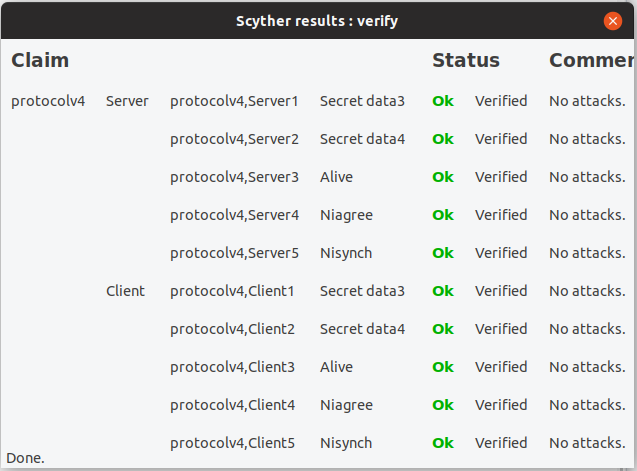
\includegraphics[width=1.0\textwidth]{figures/scyther-result.png}
		\caption{Scyther tool verification result} 
		\label{fig:scytherResult}
	\end{center}
\end{figure}

\subsection{Data Secrecy}

In the proposed protocol, sensitive information (denoted as \textit{data} in Figure~\ref{fig:scytherResult}) secrecy is achieved by encrypting each data using symmetric key $k$ algorithm which is shared between client (C) and server (S). In firmware verification protocol, vendor repository acts as a client and vendor node acts as a server. In peer-to-peer verification protocol, IoT device acts as a client and gateway acts as a server. The successful claim for the data secrecy is shown in Figure~\ref{fig:scytherResult}. The claim used in the SPDL code is:

\begin{table}[H]
	\begin{center}
		\begin{tabular}{l}
			\hline
			$\# server\ role$\\
			\boldmath{$claim(Server,Secret,data3)$} $\# server\ send\ data3$ \\
			\boldmath{$claim(Server,Secret,data4)$} $\# server\ receive\ data4$ \\
			$\# client\ role$\\
			\boldmath{$claim(Client,Secret,data3)$} $\# client\ receive\ data3$ \\
			\boldmath{$claim(Client,Secret,data4)$} $\# client\ send\ data4$ \\
			\hline
		\end{tabular}
	\end{center}
\end{table}

\subsection{Aliveness}

In the Figure~\ref{fig:scytherResult}, proposed protocol claims to ensure the server and client liveliness during the information transmission. The claim used in the SPDL code is:

\begin{table}[H]
	\begin{center}
		\begin{tabular}{l}
			\hline
			$\# server\ role$\\
			\boldmath{$claim(Server,Alive)$}\\
			$\# client\ role$\\
			\boldmath{$claim(Client,Alive)$} \\
			\hline
		\end{tabular}
	\end{center}
\end{table}

\subsection{Non-injective Agreement and Non-injective Synchronisation}

In the Figure~\ref{fig:scytherResult}, proposed protocol claims to ensure non-injective agreement and non-injective synchronisation during the information transmission. Based on \cite{nisyncandnyaggre}, non-injective agreement means all variables sent as part of the message $m$ are received as expected. Therefore, both parties will agree over the values of the variables that are sent. Non-injective syncronisation means the send event from the first run \textit{send\_1} followed by corresponding read \textit{recv\_1} and so on until the send-read event in the end of the protocol. The claim used in the SPDL code is:

\begin{table}[H]
	\begin{center}
		\begin{tabular}{l}
			\hline
			$\# server\ role$\\
			\boldmath{$claim(Server,Niagree)$}\\
			\boldmath{$claim(Server,Nisynch)$}\\
			$\# client\ role$\\
			\boldmath{$claim(Client,Niagree)$}\\
			\boldmath{$claim(Client,Nisynch)$}\\
			\hline
		\end{tabular}
	\end{center}
\end{table}

\section{Performance Analysis} 
\label{sec:performance}

In this section, comparison on performance between the proposed firmware update protocol and existing firmware update protocol are discussed. Table~\ref{tab:performanceComparison} shows the comparison of time consumption to do firmware verification protocol and peer-to-peer verification protocol between the proposed protocol and three existing firmware update protocol \cite{yohan,lee,boudguiga}.

In order to compare the computation cost between the proposed firmware update protocol and the existing protocol, the following assumptions are applied:
\begin{enumerate}
	\item The size for session key $k$ in our proposed protocol is 256 bits
	\item The symmetric encryption and decryption operation uses AES GCM with 256 bits key
	\item The one way hash function uses SHA256
	\item The key derivation function uses PBKDF2 with 1000 iterations in our proposed protocol, the output is session key $k$
\end{enumerate}
% \begin{tabular}{@{}c@{}}The time required to perform encryption (Enc) and decryption (Dec) \\ operations in symmetric cryptosystem\end{tabular}

\begin{table}[H]
	\caption{The performance comparison of four blockchain-based firmware update framework}
	\label{tab:performanceComparison}
	\begin{adjustbox}{max width=1\textwidth,center}
		\begin{tabular}{|l|l|l|}
			\hline
			\textbf{ } & \textbf{Firmware verification} & \textbf{Peer-to-peer verification} \\ \hline
			\textbf{Proposed framework} & $3T_H+2T_{KDF}+T_{symm\_enc}+T_{symm\_dec}$ & $4T_H+2T_{KDF}+3T_{symm\_enc}+3T_{symm\_dec}$\\ \hline
			\textbf{Yohan et al.~\cite{yohan}} & $6T_{sig}$ & $2T_{sig}+7T_{H}$\\ \hline
			\textbf{Lee et al.~\cite{lee}} & \begin{tabular}{@{}c@{}}$3T_{symm\_enc}+3T_{symm\_dec}+3T_{KDF}+$ \\ $10T_H+4T_{sig}$\end{tabular} & Not available \\ \hline
			\textbf{Boudguiga et al.~\cite{boudguiga}} & Not available & $4T_{sig}+T_{asymm\_enc}+T_{asymm\_dec}$ \\ \hline
		\end{tabular}
	\end{adjustbox}
\end{table}

\begin{table}[H]
	\caption{Notations used for time consumption on differing computing operations}
	\label{tab:notationtimeconsumption}
	\begin{adjustbox}{max width=1\textwidth,center}
		\begin{tabular}{cl}
			\hline
			\textbf{Notation} & \multicolumn{1}{c}{\textbf{Definition}} \\ \hline
			\boldmath{$T_H$} & The time required to perform one way hash function \\
			\boldmath{$T_{KDF}$} & The time required to perform key derivation function \\
			\boldmath{$T_{sig}$} & The time required to perform digital signature operation\\
			\boldmath{$T_{symm\_enc}$ and $T_{symm\_dec}$} & The time required to perform encryption (Enc) and decryption (Dec) operations in symmetric cryptosystem \\
			\boldmath{$T_{asymm\_enc}$ and $T_{asymm\_dec}$} & The time required to perform encryption (Enc) and decryption (Dec) operations
			in PKI cryptosystem \\
		\end{tabular}
	\end{adjustbox}
\end{table}

The execution time for the hash function (SHA256) and symmetric cryptographic operations (AES GCM) are calculated based on Crypto library benchmark using C++~\cite{cryptolib}. The benchmark compiled with Microsoft Visual C++ 2005 SP1, ran on Intel Core 2 1.83 GHz processor under Windows Vista in 32-bit mode. The execution time for the digital signature scheme and asymmetric operation (ECC 192-bits) are calculated based Yeh et al.~\cite{signatureScheme} and Tanwar et al.~\cite{asymmetricScheme}, repectively. The execution time for the cryptographic operations are shown in Table~\ref{tab:executionTime}. 

\begin{table}[H]
	\caption{The execution time of several cryptographic operations}
	\label{tab:executionTime}
	\begin{adjustbox}{max width=1\textwidth}
		\begin{tabular}{ll}
			\hline
			\textbf{Cryptographic operation} & \multicolumn{1}{c}{\textbf{Execution time}} \\ \hline
			SHA256 operation on 3200 bits of data & 28.8ms\\
			AES GCM symmetric encryption or decryption on 4000 bits of plain text & 39.21ms\\
			PBKDF2 with 1000 times iteration &  0.999ms\\
			Digital signature process (ECC 192-bits) & 11.52s \\
			ECC 192-bits asymmetric encryption or decryption & 1.064s \\
		\end{tabular}
	\end{adjustbox}
\end{table}

Based on Tabel~\ref{tab:performanceComparison}, the proposed protocol requires 166.818ms to finish firmware verification process ($3T_H+2T_{KDF}+T_{symm\_enc}+T_{symm\_dec}$). During the peer-to-peer verification process, the execution time for the proposed protocol is 352.458ms ($4T_H+2T_{KDF}+3T_{symm\_enc}+3T_{symm\_dec}$). In total, the execution time for the proposed protocol is 519.276ms.

On the contrary, the execution time of the firmware verification proposed by Lee et al.~\cite{lee} requires 46.606 seconds ($3T_{symm\_enc}+3T_{symm\_dec}+3T_{KDF}+10T_H+4T_{sig}$). Our proposed protocol has better performance regarding the execution time in the firmware verification process. The protocol proposed by~\cite{lee} requires more time to execute the digital signature process, including the digital signature verification process.

The execution time for  Yohan et al.~\cite{yohan} protocol of the firmware verification process is 69.12 seconds ($6T_{sig}$). For peer-to-peer verification,~\cite{yohan} need 23.2416 seconds, the protocol run time is 92.3616 seconds in total. Our proposed protocol also has better performance than~\cite{yohan} regarding execution time,~\cite{yohan} protocol required more time to execute the digital signature process.

The execution time for Boudguiga et al.~\cite{boudguiga} protocol of the peer-to-peer verification process is 48.208 seconds ($4T_{sig}+T_{asymm\_enc}+T_{asymm\_dec}$). Our proposed protocol has better performance than~\cite{boudguiga} regarding execution time, because~\cite{boudguiga} used digital signature and asymmetric cryptographic mechanism to secure their protocol.

\section{Discussion} 
\label{sec:discussion}

Our proposed framework leverages on the concept of skipchain to securely update the firmware in IoT environment. First, our proposed framework guarantee the secure sensitive information sharing during the process. Our proposed framework uses symmetric key algorithm to protect the sensitive information, the symmetric key algorithm uses session key produced from the shared secret from key sharing protocol. The symmetric key algorithm protects the sensitive data more computationally efficient than asymmetric key algorithm, which is more suitable for IoT environment. By using symmetric key algorithm it will also ensure the data integrity and privacy during the transmission process. Once the transaction is validated and recorded into the skipchain, this transaction can not be altered or deleted. Hence, our proposed framework could ensure end-to-end firmware integrity.

Second, our proposed framework uses skipchain, a permissioned blockchain platform, which only allows authorized vendor and gateway to join the skipchain network. Each time a vendor want to push a new firmware update, vendor need to sign the metadata with its private key. Later, the cothority member will verify the signature before put the metadata into the skipchain. Adversary can not impersonate a legitimate vendor and push a malicious firmware metadata into the skipchain, unless it has vendor's private key.

In addition, using of the long-distance backward link used in skipchain, vendor can rollback to previous firmware version efficiently if a problem occur in the new firmware (e.g. malfunction). Vendor can trace back previous stable firmware version, re-invoke the existing contract in the skipchain. It will notify the gateway to rollback based on the information in the re-invoked contract.

During the prototype implementation process, the open-source code in Github for skipchain is still under heavy development. Therefore, our prototype implementation could not use any API that calls the skipchain services. In the result, the prototype implementation uses command line interface to interact with the skipchain services. This could lead to performance issue, since we do not use direct API to call the skipchain service.
